\begin{landscape}
\section{Database \project{}}
\label{DB}
Viene riportato in questa sezione il database dell'applicativo \project{} con le tabelle e le relazioni tra esse.
\begin{figure}[!h]
	\centering
	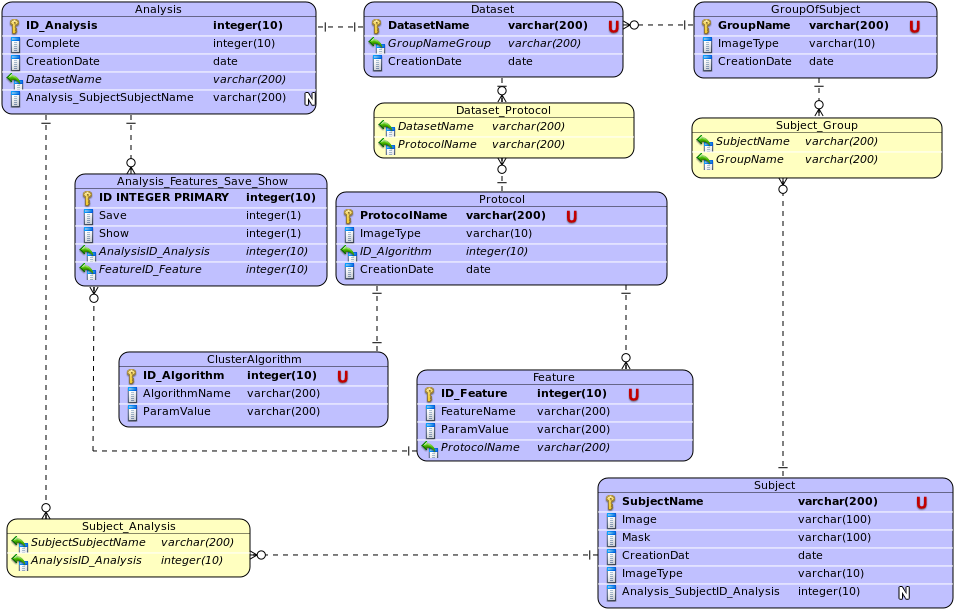
\includegraphics[width=0.7\linewidth]{./Content/Immagini/DatabaseRomeo.png}
	\caption{Struttura del database di \project{}}
	\label{DBRomeo}
\end{figure}
\end{landscape}
Il database ha il compito di mantenere lo storico delle operazioni effettuate dall'utente sul software, ovvero deve rendere disponibile tutto ciò che l'utente ha creato e modificato, ma non eliminato, dal momento dell'installazione di \project{}.

\subsection{Descrizione testuale delle tabelle}
\subsubsection{Subject}
\label{DBSub}
La tabella \textit{Subject} raccoglie tutte le informazioni necessarie per identificare un \subject{}.
\paragraph{Attributi:}
\begin{itemize}
\item \textbf{SubjectName:} \emph{varchar(200) <<PK>>} nome univoco, identificativo di un \subject{};
\item \textbf{Image:} \emph{varchar(200)} memorizza il percorso del filesystem dove è presente l'immagine associata al \subject{};
\item \textbf{Mask:} \emph{varchar(200)} memorizza il percorso del filesystem dove è presente la maschera associata al \subject{};
\item \textbf{ImageType:} \emph{varchar(10)} memorizza il tipo del \subject{};
\item \textbf{CreationDate:} \emph{date} memorizza la data e l'ora di creazione del \subject{} all'interno del programma.
\end{itemize}

\subsubsection{GroupOfSubject}
\label{DBGro}
La tabella \textit{GroupOfSubject} raccoglie tutte le informazioni necessarie per un gruppo di \subject{}.
\paragraph{Attributi:}
\begin{itemize}
\item \textbf{GroupName:} \emph{varchar(200) <<PK>>} nome univoco, identificativo di un gruppo di \subject{};
\item \textbf{ImageType:} \emph{varchar(10)} rappresenta il tipo di immagine che dovranno avere i \subject{} contenuti all'interno del gruppo;
\item \textbf{CreationDate:} \emph{date} memorizza la data e l'ora di creazione del gruppo di \subject{} all'interno del software.
\end{itemize}

\subsubsection{Dataset}
\label{DBData}
La tabella \textit{Dataset} raccoglie tutte le informazioni necessarie per un \dataset{}.
\paragraph{Attributi:}
\begin{itemize}
\item \textbf{DatasetName:} \emph{varchar(200) <<PK>>} nome univoco, identificativo di un \dataset{};
\item \textbf{CreationDate:} \emph{date} memorizza la data e l'ora di creazione del \dataset{} all'interno del software.
\end{itemize}

\subsubsection{Protocol}
\label{DBPro}
La tabella \textit{Protocol} raccoglie tutte le informazioni necessarie per un \protocol{}.
\paragraph{Attributi:}
\begin{itemize}
\item \textbf{ProtocolName:} \emph{varchar(200) <<PK>>} nome univoco, identificativo di Protocol\glossario{};
\item \textbf{ImageType:} \emph{varchar(10)} rappresenta il tipo di immagine a cui il \protocol{} verrà applicato;
\item \textbf{CreationDate:} \emph{date} memorizza la data e l'ora di creazione del \protocol{} all'interno del programma.
\end{itemize}

\subsubsection{ClusterAlgorithm}
\label{DBCla}
La tabella \textit{ClusterAlgorithm} contiene tutte le istanze degli algoritmi di clustering\glossario{} che l'utente ha creato.
\paragraph{Attributi:}
\begin{itemize}
\item \textbf{ID\_Algorithm:} \emph{Integer(10) <<PK>>} codice univoco, identificativo di una particolare istanza di algoritmo di clustering\glossario{};
\item \textbf{AlgorithmName:} \emph{varchar(200)} nome dell'algoritmo di clustering\glossario{};
\item \textbf{ParamValue:} \emph{varchar(200)} elenco dei valori dei parametri separati da punto.
\end{itemize}
Si noti che, per istanza di algoritmi di clustering\glossario{}, si intende un algoritmo di clustering\glossario{} istanziato con determinati valori dei parametri, definiti dall'utente.

\subsubsection{Feature}
\label{DBFea}
La tabella \textit{Feature} contiene tutte le istanze delle feature\glossario{} che l'utente ha creato.
\paragraph{Attributi:}
\begin{itemize}
\item \textbf{ID\_Feature:} \emph{Integer(10) <<PK>>} codice univoco, identificativo di una particolare istanza di feature\glossario{};
\item \textbf{FeatureName:} \emph{varchar(200)} nome della feature\glossario{};
\item \textbf{ParamValue:} \emph{varchar(200)} elenco dei valori dei parametri separati da punto.
\end{itemize}
Si noti che, per istanza di feature\glossario{}, si intende una feature\glossario{} istanziata con determinati valori dei parametri, definiti dall'utente.

\subsubsection{Analysis}
\label{DBAn}
La tabella \textit{Analysis} contiene tutte le informazioni relative alle analisi fatte.
\paragraph{Attributi:}
\begin{itemize}
\item \textbf{ID\_Analysis:} \emph{Integer(10) <<PK>>} codice univoco, identificativo di un'analisi;
\item \textbf{Complete:} \emph{Integer(1)} se vale \lq\lq{}1\rq\rq{}, l'analisi è stata portata a termine, altrimenti vale \lq\lq{}0\rq\rq{} e indica che l'analisi è stata interrotta;
\item \textbf{CreationDate:} \emph{date} memorizza la data e l'ora di dell'ultima analisi eseguita dal programma.
\end{itemize}

\subsubsection{Analysis\_Features\_Save\_Show}
\label{DBAnFeSaSh}
La tabella \textit{Analysis\_Features\_Save\_Show} contiene le informazioni relative a quali feature\glossario{} dell'analisi devono essere esportate e visualizzate durante l'analisi.
\paragraph{Attributi:}
\begin{itemize}
\item \textbf{ID:} \emph{Integer(10) <<PK>>} codice identificativo univoco;
\item \textbf{Save:} \emph{Integer(1)} se vale \lq\lq{}1\rq\rq{}, il risultato della feature\glossario{} viene esportato durante l'analisi, altrimenti se vale \lq\lq{}0\rq\rq{} il risultato della feature\glossario{} non viene esportato durante l'analisi;
\item \textbf{Show:} \emph{Integer(1)} se vale \lq\lq{}1\rq\rq{}, il risultato della feature\glossario{} viene visualizzato durante l'analisi, altrimenti se vale \lq\lq{}0\rq\rq{} il risultato della feature\glossario{} non viene visualizzato durante l'analisi.
\end{itemize}

\subsection{Descrizione delle associazioni}
\label{DBAss}
\begin{itemize}
\item \textbf{\lq\lq{}contain\rq\rq{}:} associazione tra \emph{GroupOfSubject} e \emph{Subject}. Un gruppo può contenere uno o più \subject{} ed un \subject{} può appartenere o meno a più gruppi;

\item \textbf{\lq\lq{}hasA\rq\rq{}:} associazione tra \emph{Dataset} e \emph{Protocol}. Un \dataset{} include uno o più \protocol{} ed un \protocol{} può essere contenuto o meno in più \dataset{};

\item \textbf{\lq\lq{}on\rq\rq{}:} associazione tra \emph{Analysis} e \emph{Subject}. Un analisi è fatta su uno o più \subject{} ed un \subject{} può essere contenuto o meno in più analisi;

\item \textbf{\lq\lq{}include\rq\rq{}:} associazione tra \emph{Dataset} e \emph{Group}. Un \dataset{} include un unico gruppo di \subject{} ed un gruppo può essere incluso o meno in più \dataset{};

\item \textbf{\lq\lq{}prevedere\rq\rq{}:} associazione tra \emph{Protocol} e \emph{ClusterAlgorithm}. Un \protocol{} contiene al più un algoritmo di clustering\glossario{} ed una particolare istanza di un algoritmo di clustering\glossario{}, può essere presente in uno o più \protocol{};

\item \textbf{\lq\lq{}calculate\rq\rq{}:} associazione tra \emph{Protocol} e \emph{Feature}. Un \protocol{} può calcolare più feature\g{} oppure nessuna ed una particolare istanza di una feature\glossario{}, può essere presente in un solo \protocol{};

\item \textbf{\lq\lq{}isDoing\rq\rq{}:} associazione tra \emph{Analysis} e \emph{Dataset}. Un'analisi viene fatta su un particolare \dataset{} ed un \dataset{} può essere presente o meno su più analisi;

\item \textbf{\lq\lq{}belongs\rq\rq{}:} associazione tra \emph{Analysis\_Features\_Save\_Show} e \emph{Analysis}. Le opzioni sulla feature\glossario{} appartengono ad un analisi, un analisi ha più opzioni sulle feature\glossario{};

\item \textbf{\lq\lq{}isOf\rq\rq{}:} associazione tra \emph{Analysis\_Features\_Save\_Show} e \emph{Feature}. Le opzioni sono di una feature\glossario{}, una feature\glossario{} può avere più opzioni;

\end{itemize}

\subsection{Progettazione logica}
\label{DBLog}
A fronte di quanto descritto precedentemente (sezione \ref{DBAss}), emerge la necessità di integrare lo schema del database con nuove tabelle. Questo è dovuto al fatto che sono presenti associazioni molti a molti. In figura \ref{DBRomeo} queste tabelle sono rappresentate in colore giallo.
\begin{itemize}
\item \textbf{Subject\_Group:} rappresenta l'associazione \lq\lq{}contain\rq\rq{} e ha come attributi le <<PK>> di \textit{Group} e \textit{Subject};

\item \textbf{Dataset\_Protocol:} rappresenta l'associazione \lq\lq{}hasA\rq\rq{} e ha come attributi le <<PK>> di \textit{Dataset} e \textit{Protocol}.

\item \textbf{Analysis\_Subject:} rappresenta l'associazione \lq\lq{}on\rq\rq{} e ha come attributi le <<PK>> di \textit{Analysis} e \textit{Subject}.
\end{itemize}
La traduzione dello schema concettuale in schema logico, ha portato all'aggiunta, in alcune tabelle, di alcuni attributi come <<FK>> che riferiscono la chiave primaria <<PK>> di altre tabelle.
\begin{itemize}
\item \textbf{DatasetName:} <<FK>> in \textit{Analysis} che rappresenta il \dataset{} su cui viene fatta l'analisi;
\item \textbf{GroupName:} <<FK>> in \textit{Dataset} che rappresenta il gruppo di \subject{} contenuto nel \dataset{};
\item \textbf{ProtocolName:} <<FK>> in \textit{Feature} che rappresenta il \protocol{} a cui è associata l'istanza della feature\glossario{};
\item \textbf{ID\_Algorithm} <<FK>> in \textit{Protocol} che rappresenta l'eventuale algoritmo di clustering\glossario{} associato al \protocol{};

\item \textbf{ID\_Feature} <<FK>> in \textit{Analysis\_Features\_Save\_Show} che rappresenta la feature\glossario{} da esportare o visualizzare durante l'analisi;
\item \textbf{ID\_Analysis} <<FK>> in \textit{Analysis\_Features\_Save\_Show} che rappresenta a quale analisi la feature\glossario{} da esportare o visualizzare è associata;
\end{itemize}